\section{Optoelectronic coupling}

The non-interacting system displays valley selective optical excitations.
Light of a particular polarization only couples to one valley.
Since the superconducting state is
a coherent condensate admixing the two valleys,
we address whether pair-breaking displays similar valley selectivity.
In particular, we explore whether or not the two quasiparticles generated
by circularly polarized light, with total energy larger than
$E_g + Δ_{\vK}$, occupy opposite valleys,
with one in the conduction band and the other in the valence band.

The optical excitations arise from the Berry curvature,
which acts as an effective angular momentum.
The electromagnetic potential $\vc{A}$,
with polarization vector $\vc{ϵ}$,
is introduced using minimal coupling,
$H_{τ {\s}}^{ν ν'} \ofK
→ H_{τ {\s}}^{ν ν'} \of{\vK + e \vc{A}}$,
where, in the dipole approximation,
$\vc{A} = 2 \re{\vc{ϵ} A_0 e^{- i ω t}}$.
This yields a perturbed Hamiltonian
$H → H + H^A$, where
$H^A = H' e^{- i ω t} + H'^† e^{i ω t}$,
with
\begin{multline}
  H'
  = ∑_{\vK, τ, {\s}}
    H'_τ
    {d^-_{τ {\s}}}^† \ofK
    d^+_{τ {\s}} \ofK \\
  - ∑_{\vK, τ, {\s}}
    H'_{-τ}
    {d^+_{τ {\s}}}^† \ofK
    d^-_{τ {\s}} \ofK,
\end{multline}
and
$H'_τ
= a t e A_0
\left( τ \vc{\hat{x}} + i \vc{\hat{y}} \right) · \vc{ϵ}$.
The transition rate is proportional to the modulus-squared
of the optical matrix elements,
$\vc{P}_{τ {\s}}^{n n'} \ofK$,
defined by
\begin{equation}
  H^A
  = ∑_{\substack{\vK, τ, {\s} \\ n, n'}}
    \frac{e A_0}{m_0}
    \vc{ϵ} · \vc{P}_{τ {\s}}^{n n'} \ofK
    {c_{τ {\s}}^n}^† \ofK
    c_{τ {\s}}^{n'} \ofK.
\end{equation}
For circularly polarized light, in the absence of superconductivity,
$\vc{ϵ}_± = \left( \vc{\hat{x}} ± i \vc{\hat{y}} \right) / \sqrt{2}$ and
\begin{equation}
  \label{eq:optical}
  \vc{ϵ}_± · \vc{P}_{τ {\s}}^{+ -} \of{\vK}
  = ∓ τ \sqrt{2} a t m_0
    e^{± i ϕ}
    \sin^2 {\frac{\fnTheta{∓ τ}}{2}}.
\end{equation}

\begin{figure}
  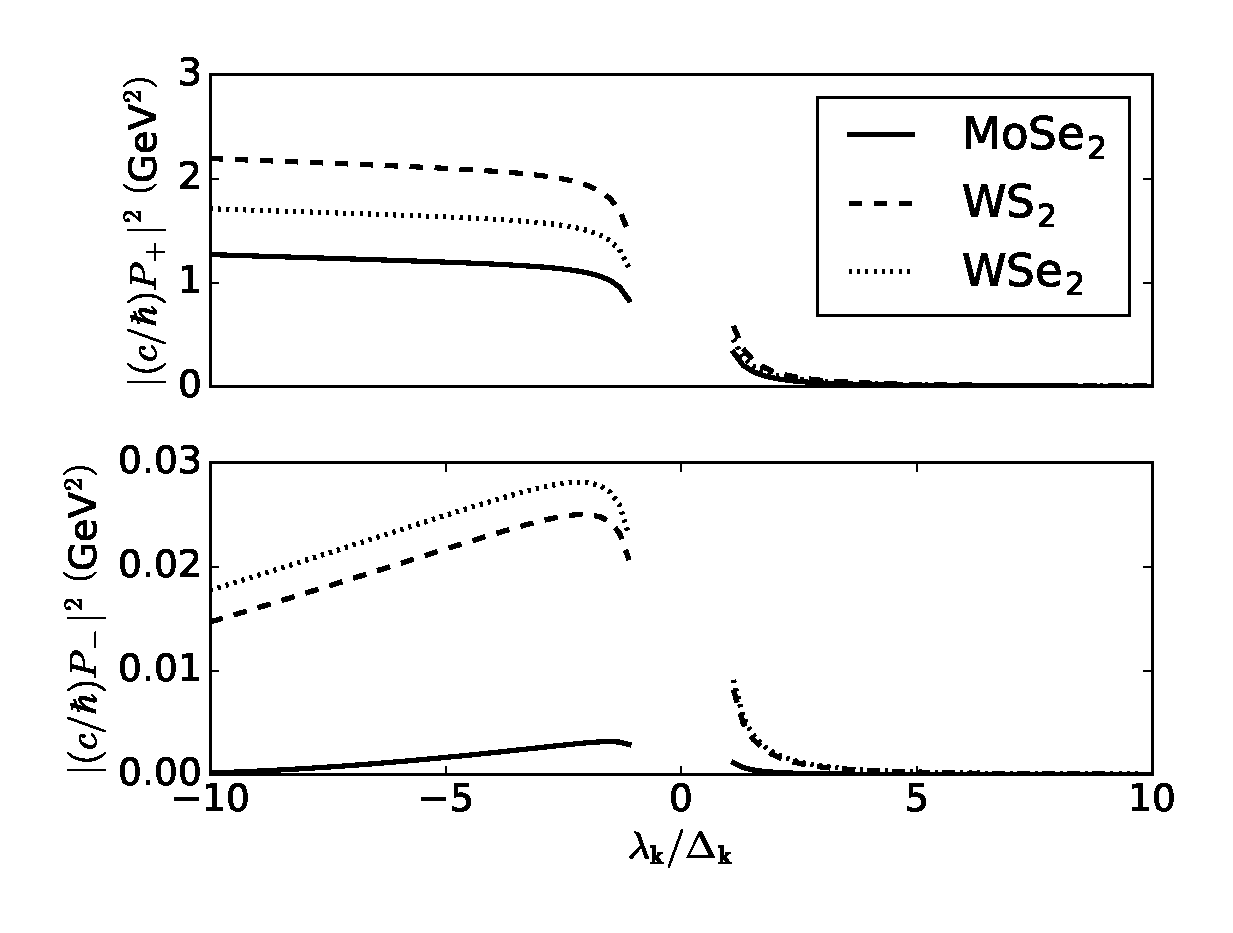
\includegraphics[width=\columnwidth]{figures/optical-transitions-bcs}
  \caption{%
    Optical transition rate matrix elements
    $\left| P_± \right|^2$
    in the superconducting phase
    as a function of the ratio of the quasiparticle energy
    $λ_{\vK}$ to the superconducting gap $Δ_{\vK}$.
    Material parameters for \ce{MoSe2}, \ce{WS2}, and \ce{WSe2}
    are given in~\cite{PhysRevLett.108.196802}
    and a gap of $Δ_{\vK} = \SI{7.5}{\milli\electronvolt}$
    is chosen for illustrative purposes.
    The order-of-magnitude contrast between
    $\left|P_+\right|^2$ and $\left|P_-\right|^2$
    causes the optical-valley selectivity.
  }\label{fig:optical}
\end{figure}

The transition rate matrix elements
for optical excitations from the BCS ground state
are given by \cref{eq:optical}
multiplied by a coherence factor $\sin {β_{\vK}}$.
Since $\fnTheta{-} - \fnTheta{+} = τ π$,
switching either the valley or polarization transforms
$\sin → \cos$ in \cref{eq:optical}, giving matrix elements
$\abs{P_±} = \abs{\vc{ϵ}_± · \vc{P}_{++}^{+ -} \ofK \sin {β_{\vK}}}$
corresponding to matching ($P_+$) or mismatching ($P_-$)
polarization-valley indexes.
For a given valley, a chosen polarization of light couples more strongly
than the other, as is evident comparing $\abs{P_+}^2$ to $\abs{P_-}^2$
and shown in \cref{fig:optical}.
For incident light with energy $E_g + \abs{λ_{\vK}}$,
right circularly polarized light ($+$) has a higher probability
of promoting a quasiparticle to the right conduction band,
as reflected in the larger matrix element $\abs{P_+}^2 ≫ \abs{P_-}^2$.
As depicted in \cref{fig:optical-excitation},
the partner of the Cooper pair is in the valence band in the opposite valley.
The other valley has the opposite dependence on polarization.

This key new result opens the door for valley control of excitations
from a coherent ground state.
For example, the two quasiparticles have the same charge and Berry curvature
(see below).
In the presence of an electric filed,
they both acquire the same transverse anomalous velocity.
Thus, in contrast to the response in the normal state,
an anomalous Hall effect is anticipated
with no accompanying spin current.

\begin{figure}
  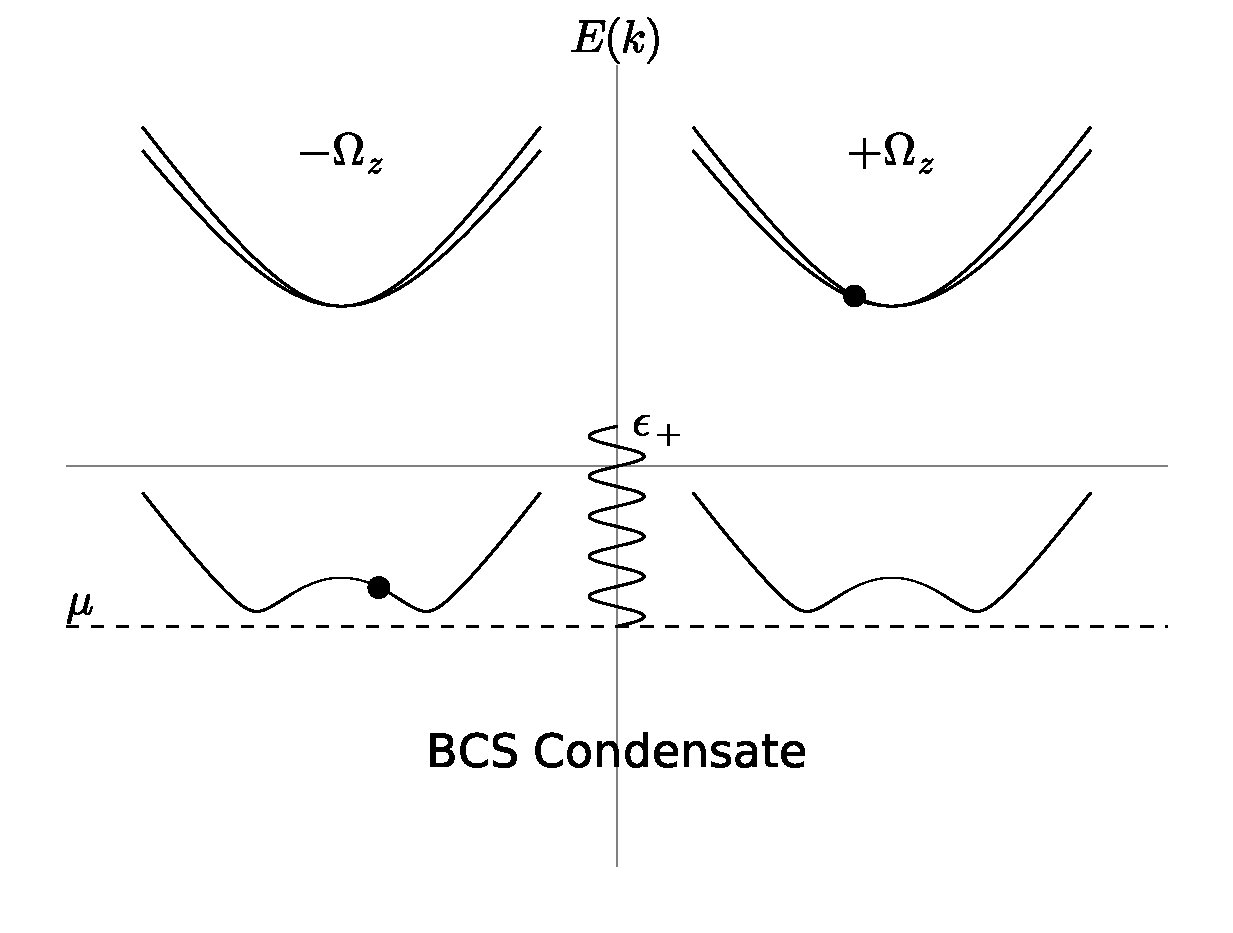
\includegraphics[width=\columnwidth]{figures/bcs-excitation}
  \caption{%
    Pair-breaking by right circularly polarized light
    leads to an electron in the conduction band of the right valley
    and a partner in the valence band of the left valley.
    The valleys interchange for left circularly polarized light.
  }\label{fig:optical-excitation}
\end{figure}
